\chapter{Wissensrepräsentationsformen}
\label{chap:wissensrepFormen}

Nachdem im letzten Kapitel etwas über die Grundlage der Graphen sowie Graphdatenbanken aufgezeigt wurde, soll hier auf konkrete Repräsentationsformen von Wissen eingegangen werden.
In der Wissensmodellierung (Knowledge Engineering) gibt es verschieden Wissensrepräsentationsformen um die Wissen in wissensbasierten Systemen formal abzubilden. Die so gesammelten Informationen werden als Wissensdatenbank respektive Wissensbasis bezeichnet.~\cite{wikiWissensrep}

Das folgende Kapitel basiert auf~\cite{laemmel} und beschreibt einige der klassischen Wissensrepräsentationsformen.

Semantische Netze, Wissensnetze und Frames gehören zu den üblichen Wissensrepräsentationsformen. Dabei stehen die konkreten Objekte im Vordergrund und nicht, wie zum Beispiel bei Regeln, die Zusammenhänge und die logischen Abhängigkeiten.

Semantische Netze und Frames versuchen das menschliche Gedächtnis in adäquater Form abzubilden. Ursprünglich wurden Sie vor allem zur Analyse von Wörtern und Sätzen verwendet. Ein weiterer Punkt ist die einfach verständliche Darstellung von Klassen und deren Beziehungen. Zudem haben die Konzepte der semantischen Netze und Frames die Entwicklung der objektorientierten Programmierung beeinflusst.

\section{Semantische Netze}
\label{sec:wissensrepFormen_semantischeNetze}

Eine zusammengehörige Gruppe von Objekten wird als Klasse bezeichnend. Ein einzelnes Objekt nennt sich auch Individuum. Zwischen den Objekten untereinander, zwischen Objekten und Klassen oder zwischen Klassen untereinander gibt es Beziehungen. Es kann zwischen folgenden Beziehungen unterschieden werden:

\begin{itemize}
    \item "`ist eine"' Relation

        Es handelt sich um Ober- und Unterklassen.

        Beispiel: \textit{Ein Baum ist eine Pflanze.}

    \item "`Instanz von"' Relation

        Die Relation beschreibt die Beziehung einer konkreten Instanz zu ihrer Klasse.

        Beispiel: \textit{Birke ist eine Instanz der Klasse Baum.}

    \item Eigenschaft

        Klassen und Objekte haben Eigenschaften.

        Beispiel: \textit{Pflanzen erzeugen Sauerstoff.}
\end{itemize}

Eigenschaften sind transitiv: Ist also ein Hund ein Tier und ein Tier ein Lebewesen, ist auch ein Hund ein Lebewesen. Ausserdem halten sich Eigenschaften an das Gesetz der Vererbung. Braucht also ein Tier Sauerstoff, braucht auch ein Hund Sauerstoff.

In semantischen Netzen werden Objekte und Klassen als Knoten abgebildet. Beziehungen und Eigenschaften werden als Kanten dargestellt.
Einige Ausdrucksformen wie Existenzaussagen und Oder-Aussagen können mit semantischen Netzen nicht abgebildet werden. Obwohl sich nur zweistellige Beziehungen abbilden lassen, sind komplexe Abbildungen, wie zum Beispiel das Modellieren einer Aktion, möglich.

\section{Frames}
\label{sec:wissensrepFormen_frames}

In Frames werden die wesentlichen Charakteristika eines Objekts als Eigenschaften abgebildet und zusammengefasst. Dabei unterstützten Frames die Konzepte der Hierarchie und der Vererbung. Zudem können Frames auch generische Informationen wie Defaults, also Standartwerte, und Wertebeschränkungen (Listen) enthalten.

\begin{lstlisting}[caption={Beispiel eines Frames anhand einer Reise.}]
    frame Abenteuerreise is a Reise :
        default hatReiseleiter is true
    instance `Dschungeltrip' is a kind of Abenteuerreise :
        anbieter is dernettereiseanbieter
        and typ is abenteuer
        and kosten is 1000.
    constraint preise
        when the typ of an Abenteuerreise changes to X
        then check that X is {dschungel or abenteuer or nevernkitzel or natur}
        otherwise write( `Der Typ der Reise wurde nicht geändert' )
        and nl.
\end{lstlisting}

\section{Wissensnetze}
\label{sec:wissensrepFormen_Wissensnetze}
Bei Wissensnetzen handelt es sich um eine Art der Wissensrepräsentation, welche die Konzepte der semantischen Netzte verwenden. Dabei wird eine objektorientierte oder Frame-Darstellung des Wissens integriert. Zusätzlich erfolgt eine grafische Darstellung mittels Topic Maps. Diese wird auch Wissenslandkarte genannt. 

Die Entfernung zweier Begriffe in der Wissenslandkarte bilden deren inhaltliche Nähe ab. Es werden also die semantischen Beziehungen der Begriffe verwaltet. Dies ist eine grosse Unterstützung der semantische Suche.

Wie in den semantischen Netzen werden Instanzen und Klassen in den Knoten abgebildet. Zusätzlich wird das Problem der Mehrfachvererbung umgangen, indem das Konzept der Rollen eingeführt wird. Klassen werden so ausgebaut, das eine Instanz eine bestimmte Rolle annehmen kann.

Wissensnetze haben sämtliche Voraussetzungen um effektives Wissensmanagement zu erreichen. Dafür muss das Wissen aber immer aktuell und entsprechend umfangreich sein.

\newpage

\noindent\rule[1ex]{\textwidth}{1pt}
\begin{wrapfigure}{l}{0.1\textwidth}
    \vspace{-2pt}
    
\includegraphics[width=0.1\textwidth]{bilder/owl.png}
\end{wrapfigure}\\
Ein sehr wichtiger und zeitintensiver Teil des Knowledge Engineerings ist die tatsächliche Modellierung. Also die Überlegung ob eine abzubildende Information ein Objekt, eine Instanz oder eine Eigenschaft ist, oder, ob sie gar als Regel abgebildet werden kann. Regeln werden im Kapitel~\ref{chap:swrl}~\refname{chap:swrl} genauer erläutert. Uns scheint an dieser Stelle aber wichtig zu erwähnen, dass das semantischen Netz ein sehr gutes Hilfsmittel war, um einen Überblick über die Informationen und ihre Verwendbarkeit zu erhalten.
An unserem konkreten Beispiel könnte dies folgendermassen aussehen:

\begin{figure}[H]
\centering \rotatebox{0}{\scalebox{0.5}[0.5]{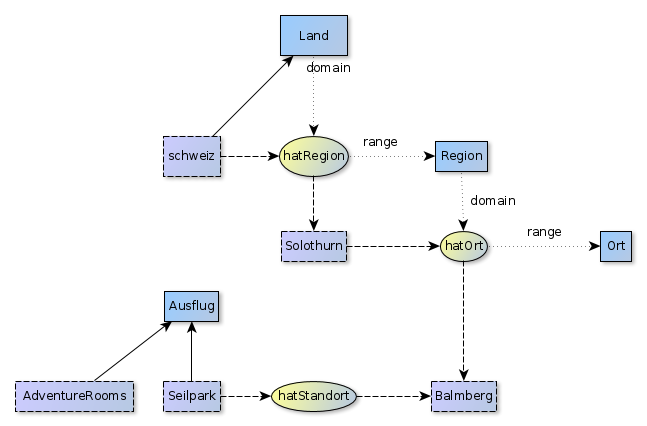
\includegraphics{bilder/beispiel_semantisches_netz.png}}}
\caption{Abbildung von Wissen mittels einem semantischen Netz.\label{fig:semantischesNetz}\protect\footnotemark}
\end{figure}
\footnotetext{Eigene Darstellung mittels yEd}

Die obige Abbildung mag auf den ersten Blick simpel erscheinen, wie aber bereits vorher erwähnt, handelt es sich um einen Übersicht der Informationen. Würde man das Wissen direkt so in die Semantische Datenbank übertragen, wäre diese nicht viel mächtiger als eine traditionelle Wissensspeicherung. Dies führen wir zu einem späteren Zeitpunkt noch genauer aus.\\

\vspace{0.1pt}
\noindent\rule[1ex]{\textwidth}{1pt}


% Einträge im Verzeichnis erscheinen lassen ohne hier eine Referenz einzufügen
%\nocite{kopka:band1}
